\section{Der ATLAS-Detektor}
\subsection{Teilchen in Materie}
\paragraph{Bethe-Bloch}
Um den Aufbau des \atlas-Detektors zu verstehen müssen wir zunächst verstehen wie Teilchen mit Materie interagieren. Geladene Teilchen die sich durch Materie bewegen verlieren durch Interaktionen mit den Atomen an Energie. Diese Interaktionen umfassen Bremsstrahlung bei hohen Energien, Ionisation bei mittleren Energien und Anregung von Atomen bei geringen Energien. Der Energieverlust in Abhängigkeit von der Energie des Teilchens ist in Abb. \ref{fig:bethe} dargestellt. Für schwere geladene Teilchen, wie z.B. das Myon wird der Energieverlust durch Ionisation durch die Bethe-Bloch Formel beschrieben\cite{Passage_through_matter}. Der Energieverlust durch Ionisation hängt dabei nicht von der Masse des Teilchens ab und ist nur durch die Materialbeschaffenheit und die Geschwindigkeit und Ladung des Teilchens eindeutig bestimmt. 
\begin{figure}
\centering
\includegraphics[scale=0.7]{./input/bethe.pdf}\caption{Energieverlust pro Strecke (Stopping power) aufgetragen gegen den Impuls eines Myons. Der Verlust durch Ionisation findet in einem Bereich von 10~Mev und 100~GeV statt\cite{Passage_through_matter}.}\label{fig:bethe}
\end{figure}
Um diesen Mittelwert ist der Energieverlust nach der Landau-Verteilung verteilt.
\begin{figure}
\centering
\includegraphics[]{./input/landau.pdf}\caption{Landau-Verteilung des nach Bethe-Bloch berechneten Energieverlusts.\cite{Passage_through_matter}}\label{fig:landau}
\end{figure}
\paragraph{Elektronen und Photonen}\label{sec:emschauer}
Photonen und Elektronen verlieren ihre Energie in Materie hauptsächlich durch Bremsstrahlung (Elektronen), und Paarerzeugung (Photonen). Weil ein Elektron durch Bremsstrahlung Photonen aussendet und ein Photon durch Paarerzeugung Elektronen erzeugt sind beide Vorgänge eng miteinander verbunden. Eine Materialkonstante, die eine wichtige Rolle spielt ist die Strahlungslänge $X_0$. Sie entspricht der Länge nachdem ein Elektron in Materie alles bis auf $1/e$ seiner Energie abgegeben hat\cite{Passage_through_matter}. Gleichzeitig ist es $7/9$ der mittleren freien Weglänge eines Photons in diesem Material. Die aufeinander folgende Bremsstrahlung und Paarerzeugung von Photonen und Elektronen führt zu einer Teilchenkaskade. Die Teilchenkaskade endet, wenn die kritische Energie $E_c$ erreicht wird. Dies ist die Energie der Elektronen bei der der Energieverlust durch Ionisation überwiegt, somit fast keine Bremsstrahlung mehr auftritt.

\section{Silizium Detektor}
Die innerste Schicht des \atlas-Detektors ist der Spurdetektor. Er setzt sich aus drei verschiedenen Halbleiterdetektoren zusammen: Dem innersten Pixel-Detektor, dem Silizium-Streifen-Detektor und dem Übergangsstrahlungsdetektor\cite{atlas_build}. Ihre Funktionsweise ähnelt sich jedoch. Trifft ein geladenes Teilchen auf eine Zelle eines Halbleiter-Detektors, so ionisiert es die Atome des Kristalls, die frei werdenden Elektronen werden in das Leitungsband des Halbleiters absorbiert. Was man detektiert, ist der Strom der dadurch erzeugt wird. Durch $\delta$-Elektronen, Elektronen die durch den Stoß genug Energie bekommen um selbst Atome zu ionisieren, ist es möglich ein Signal in mehreren Pixeln zu erhalten. In diesem Fall verbessert sich die Auflösung, da man aus der Signalstärke der einzelnen Pixel den Eintrittsort des ursprünglichen ionisierenden Teilchens genauer bestimmen kann als es das Signal eines einzelnen Pixel erlauben würde. Die Spur eines Teilchens kann gemessen werden, da ein ionisierendes Teilchen Hits in aufeinanderfolgenden Schichten des inneren Detektors hinterlässt. Dabei wird der innere Detektor von einem Magnetfeld in Richtung der Strahlachse durchsetzt, sodass die Teilchenbahnen gekrümmt sind. Aus der Krümmung lässt sich der Impuls eines geladenen Teilchens bestimmen. Der Aufbau des inneren Detektors ist in Abb. \ref{fig:inner} zu sehen.
\begin{figure}
\centering
\includegraphics[scale = 0.5]{input/innerdetector.jpg}\caption{Aufbau der Halbleiterdetektoren des \atlas-Detektors. Pixel-detectors (Pixel-Detektor), Barrel- und Endcap-transition-radiation-tracker (Übergangsstrahlungsdetektoren), Barrel- und Endcap-semiconductor-tracker (Siliziums-Streifen-Detektor) \cite{atlas_build}.}
\end{figure}


\section{Kalorimeter}\label{sec:calori}
\subsection{Prinzip}
Die nächst äußere Schicht des \atlas sind die beiden Kalorimeter. Das elektromagnetische (EM) Kalorimeter innen und das hadronische Kalorimeter außen. In den Kalorimetern wird die kinetische Energie eines Teilchens gemessen. Das EM Kalorimeter misst die Energie von geladenen Teilchen, vor allem Elektronen, und Photonen. Die Wechselwirkungen von Elektronen und Photonen mit Materie wurden bereits in \ref{sec:emschauer} beschrieben. Das hadronische Kalorimeter detektiert die bei der Interaktion von Hadronen mit Materie entstehenden Elektronen, auf dieselbe Weise. Dabei wird berücksichtigt, dass nur ein Teil der Energie des Hadrons durch einen elektromagnetischen Schauer deponiert wird.
Bei einem Sampling-Kalorimeter wechseln sich Absorberschichten, die den Schauer erzeugen, und Messschichten, die die deponierte Energie messen, ab, wohingegen bei homogenen Kalorimetern das Absorbermaterial gleichzeitig das signalerzeugende Material ist (z.B. durch Cherenkov-Strahlung in Bleiglas). Die Messschichten können zum einen wie Ionisationskammern aufgebaut sein, zum anderen können aber auch Szintillatoren verwendet werden die durch ionisierende Strahlung Licht erzeugen, welches dann gemessen werden kann. Der erste Fall findet im EM Kalorimeter des \atlas Anwendung\cite{Aad:2014una} und der zweite Fall im hadronischen Kalorimeter desselben\cite{Meyer:2013joa}. Die Materialien, die beim hadronischen Kalorimeter verwendet werden, müssen so gewählt sein, dass in etwa die gleiche Energie des einfallenden Hadrons über elektromagnetische Schauer deponiert wird wie über hadronische, um eine möglichst genaue Bestimmung der Energie zu gewährleisten.
Aus der Position des Schauermaximums lässt sich die kinetische Energie des einfallenden Teilchen bestimmen. 
Die relative Auflösung wird dabei mit steigender kinetischer Energie besser. In Abb. \ref{fig:emcalori} ist der Aufbau des EM Kalorimeters zu sehen.

\begin{figure}
\centering
\includegraphics[scale=0.45]{input/LAr_Labeled.pdf}\caption{Das elektromagnetische Kalorimeter des \atlas-Detektors. Das signalerzeugende Material ist flüssiges Argon(liquid Argon(LAr))\cite{Aad:2014una}. Das Kalorimeter besteht aus einem Mantel-Teil (Barrel) und Endplatten (Endcap) um möglichst viel Fläche abzudecken.}
\end{figure}

% \subsection{Hadronische Schauer}
% Hadronische Schauer entstehen wenn hochenergetische Hadronen mit Materie wechselwirken. Durch Interaktionen mit Atomkernen entstehen neue Hadronen, die ähnlich wie die elektromagnetischen Schauer eine Kaskade an neu entstehenden Hadronen erzeugen. Allerdings geht nur ein Teil der Energie des ursprünglichen Hadrons in den hadronischen Schauer über. In einem Hadronischen Schauer entstehen unter anderen Mesonen Pionen, die zu zwei Photonen zerfallen können. Diese Photonen wiederrum rufen einen elektromagnetischen Schauer hervor. Im Gegensatz zu Kernreaktionen lassen sich die Interaktionen zwischen Photonen, Elektronen und Materie über Ionisation messen. Deswegen werden aus dem elektromagnetischen Teil eines hadronischen Schauers die tatsächlich deponierte Energie berechnet. Um statistische Schwankungen zu minimieren muss dafür das Kalorimeter so gebaut sein, dass die Energie, die durch den hadronischen Teil deponiert wird, der Energie, die durch den elektromagnetischen Teil deponiert wird, entspricht.

\section{Gas-Detektoren}
\subsection{Lawinen-Bildung}
Hinter den Kalorimetern des \atlas befinden sich die Myondetektoren. Es handelt sich dabei um Ionisationskammern. Ionisationskammern bestehen im Allgemeinen aus einer Anode und einer Kathode zwischen denen sich ein Gas als Ionisationsmedium befindet. Trifft ein ionisierendes Teilchen in die Kammer, so schlägt es Elektronen aus den Gasmolekülen heraus. Diese Elektronen werden durch die Spannung zwischen Anode und Kathode beschleunigt, sodass sie selbst wieder genug kinetische Energie haben um selbst Moleküle zu ionisieren. Ein einfallendes Teilchen produziert auf diese Weise eine Elektronen-Lawine, die als messbarer Strom zwischen Anode und Kathode nachgewiesen werden kann. In Abhängigkeit von der angelegten Spannung ist das Signal entweder proportional zu der durch das ursprünglich einfallende Teilchen verursachten Ionisation, oder für jedes Teilchen gleich. Der letztere Fall tritt zum Beispiel beim Geiger-Müller-Zählrohr auf, bei dem lediglich gemessen wird ob ein ionisierendes Teilchen im Zählrohr aufgetroffen ist oder nicht. Für die Teilchenphysik sind vor allem Detektoren von Nutzen, die ein zur Ionisation proportionales Signal liefern, da in diesem Fall zwischen Teilchen unterschieden werden kann.
% \subsection{Die Multi-Wire-Proportional-Chamber(MWPC)}
% Die MWPC ist eine Ionisationskammer bestehend aus vielen einzelnen Anodendrähten und Kathodenplatten die parallel zur Ebene der Drähte angeordnet sind(siehe Abb. \ref{fig:MWPC}). Durch die Verwendung mehrerer Anodendrähte ist es möglich den Einschlagsort des Teilchens in der Achse senkrecht zu den Anodendrähten zu bestimmen. Verwendet man mehrere Ebenen so lassen sich auch zwei- und dreidimensionale Messungen durchführen.
% \begin{figure}
% \centering
% 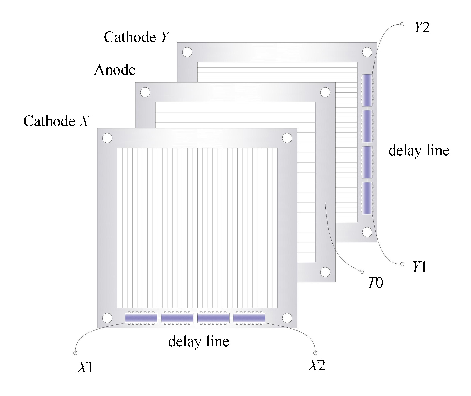
\includegraphics[]{./input/MWPC.eps}\caption{Schematische Darstellung einer MWPC\cite{Tang:2013daa}.}\label{fig:MWPC}
% \end{figure}
\subsection{Driftkammer}\label{sec:drift}
Die Myondetektoren des \atlas sind Driftröhren. Diese sind ein spezielle Art von Driftkammern. 
Driftkammern nutzen eine konstante Driftgeschwindigkeit der durch Ionisation freiwerdenden Elektronen aus, um aus dem Zeitpunkt des durch die Elektronen entstehenden Signals den genauen Abstand des Teilchendurchgangs von der Anode zu bestimmen. Vorraussetzung dafür ist ein möglichst homogenes elektrisches Feld und die Kenntnis über den Zeitpunkt des Eintreffens des ionisierenden Teilchens.  
Driftröhren sind längliche Driftkammern, bei denen ein Anodendraht von einem Kathodenmantel umgeben ist. Zwischen Draht und Mantel befindet sich das Medium. 
Im \atlas werden Drifttubes dabei leicht versetzt geschichtet eingesetzt, sodass eine gute Auflösung in den beiden Achsen senkrecht zu den Drifttubes möglich wird\cite{2010EPJC...70..875A}. Den Auftreffort des Teilchen in der Achse parallel zu den Drifttubes kann man über die Stärke des Signals an beiden Enden des Drifttubes bestimmen. Die Ionisationslawine fließt in beide Richtungen des Anodendrahtes ab, die Stärke des Signals jedoch hängt jedoch von der zurückgelegten Strecke ab. Aus dem Verhältnis der Signale lässt sich berechnen an welcher Stelle des Drahtes die Ionisation stattgefunden hat.
In den Myonkammern des \atlas herrscht ein toroidales Magnetfeld, sodass Myonen immer in Richtung der Strahlachse abgelenkt werden\cite{2010EPJC...70..875A}. Auch aus ihrer Bahn lässt sich ihr Impuls bestimmen. In Abb. \ref{fig:muon} ist die Anordnung von aus Drifttubes zusammengesetzten Platten am \atlas-Detektor zu sehen.

\begin{figure}
\centering
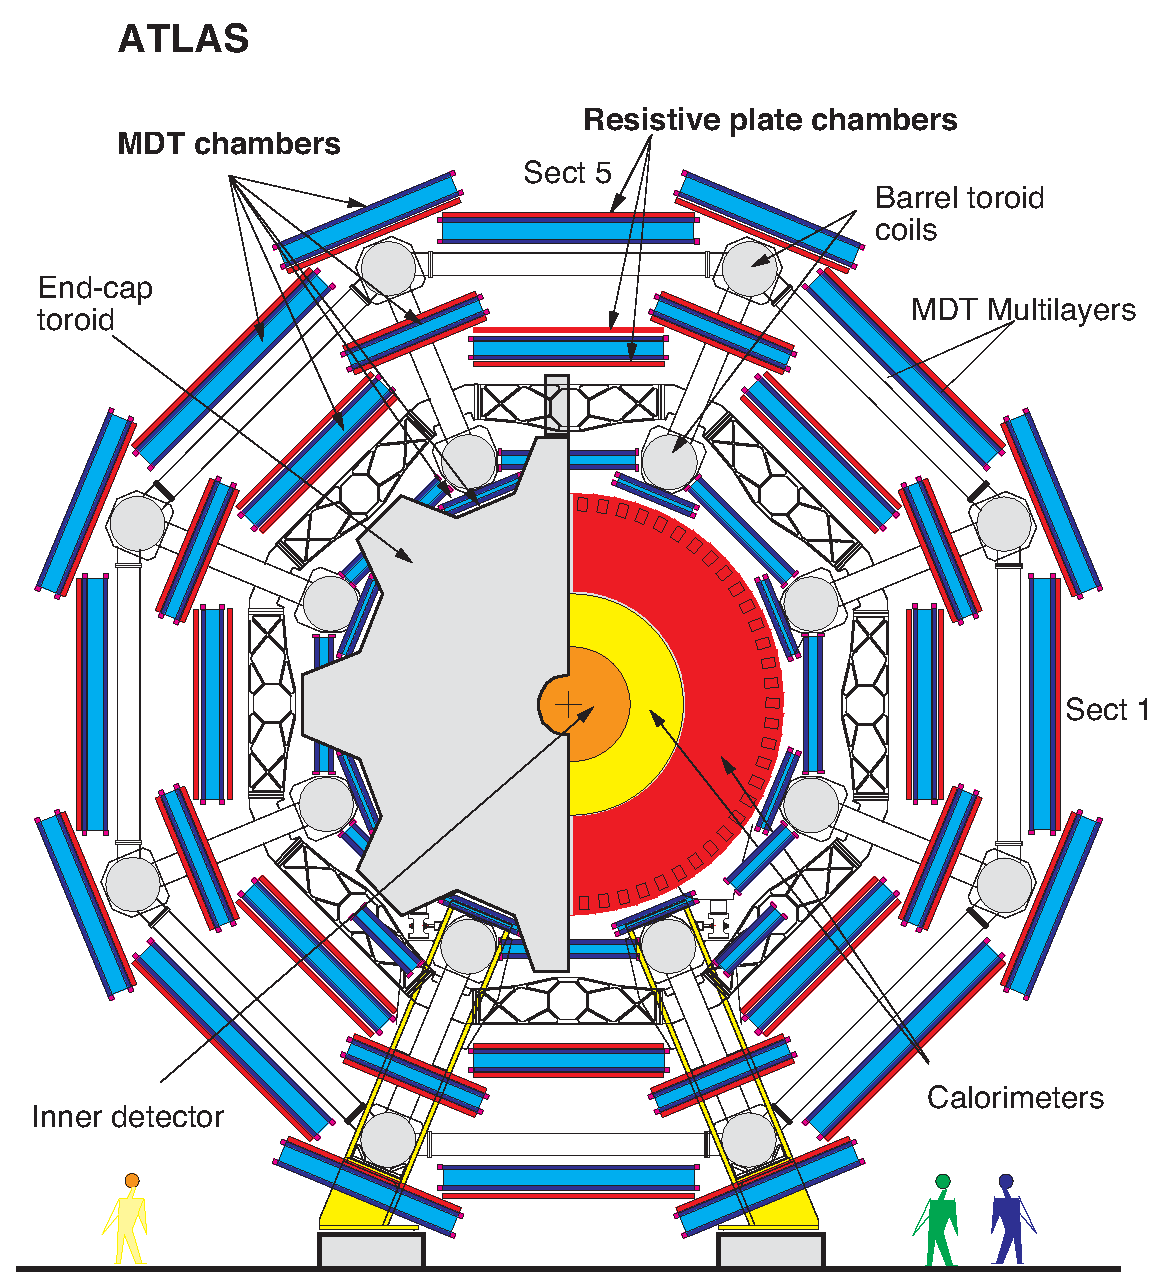
\includegraphics[scale=0.4]{input/Fig1a.eps}\caption{Anordnung der Myon-Detektoren im \atlas-Experiment. Platten bestehend aus Lagen von Drifttubes (MDT-Chambers) sind blau dargstellt\cite{2010EPJC...70..875A}.}\label{fig:muon}
\end{figure}

% \subsection{Time-Projection-Chamber (TPC)}
% Die TPC funktioniert ähnlich wie die Driftkammer mit dem Unterschied, dass in der TPC die Anode eine Fläche ist, die aufgeteilt in Anodensegmente ist. In jedem der Segmente lässt sich unabhängig von benachbarten Segmenten ein Strom messen. Durchquert ein Teilchen die TPC so hinterlässt es eine Spur aus Ionen und Elektronen. Die Elektronen driften nun zur Anode hin, aus den Zeitpunkten zu denen die Elektronen auf die Anodensegmente auftreffen lässt sich nun die gesamte Bahn des Teilchens rekonstruieren. Der Abstand der Teilchenbahn zur Anode wird also auf die Zeit, die Elektronen zu Anode brauchen, projiziert.


\section{Teilchen Identifikation}
Teilchen können auf verschiedene Weisen identifiziert werden. Am einfachsten ist die Identifikation durch ihre Interaktion mit dem Detektor. Geladene Teilchen hinterlassen eine Spur im Spurdetektor, und erzeugen einen Schauer im elektromagnetischen(EM) Kalorimeter. Anhand der Krümmung der Spur kann die Ladung und der Impuls des Teilchens bestimmt werden. Auf diese Weise werden Elektronen detektiert. Photonen bilden keine sichtbare Spur im Spurdetektor, erzeugen jedoch einen Schauer im elektromagnetischen Kalorimeter, können also auf diese Weise identifiziert werden. Geladene Hadronen wie z.B. das $\pi^+$-Meson, hinterlassen sowohl eine Spur im Spurdetektor als auch einige Hits im EM Kalorimeter. Zusätzlich erzeugen sie einen Schauer im hadronischen Kalorimeter. Neutrale Hadronen wie das Neutron hinterlassen keine Spur im Spurdetektor, und sind auch im EM Kalorimeter nicht messbar. Allerdings erzeugen sie einen Schauer im hadronischen Kalorimeter. Somit sind sie auf diese Weise nachweisbar. Ein Problem stellt das Myon dar, was trotz Ladung, nicht durch die Kalorimeter gestoppt wird. Myonen werden durch spezielle Myonenkammern detektiert, die die äußersten Bestandteile eines Detektors bilden. Bei dem Myonenkammern handelt es sich um Ionisationskammern. Beim \atlas-Detektor sind dies Drifttubes. Außer den Myonen hinterlassen keine anderen Teilchen Spuren in den Myonkammern, da sie bereits in den Kalorimetern gestoppt wurden.
Neutrinos können nicht detektiert werden, da sie nur schwach wechselwirken. Deswegen können Neutrinos nur aus der transversalen Impulserhaltung rekonstruiert werden, wobei deren Energie als \emph{missing transverse energy} \MET bezeichnet wird.\\ \noindent
Andere Möglichkeiten Teilchen zu identifizieren umfassen den Energieverlust eines Teilchen ins Materie, wobei die Ladung des Teilchens aus der Bethe-Bloch-Formel bestimmt werden kann, Time-of-Flight Detektoren, die die Zeit messen die ein Teilchen braucht um sich von einem Interaktionspunkt zu einem zweiten zu bewegen, und Cherenkov-Detektoren. 


